\appendix

\chapter{An Example: TPC-H Query 6}
\label{appendix:full-query}

TPC-H query 6 is arguably the simplest of the 22 queries in the TPC-H benchmark. In this section, we will show how our query processor evaluates this query, and the various intermediate representations that are reached.

Figure \ref{fig:q6-sql} shows the SQL query that is inputted. This corresponds to step 1 in figure \ref{fig:translation-process}.

\begin{figure}[H]
    \centering
    \begin{tabular}{|c|}
    \hline
    \begin{lstlisting}[language=SQL]
SELECT
    sum("l_extendedprice" * "l_discount") as "revenue"
FROM
    "lineitem"
WHERE
    "l_shipdate" >= date '1994-01-01'
    AND "l_shipdate" < date '1994-01-01' + interval '1' year
    AND "l_discount" between 0.06 - 0.01 AND 0.06 + 0.01
    AND "l_quantity" < 24
    \end{lstlisting} \\
    \hline
    \end{tabular}
    \caption{TPC-H query 6 in SQL}
    \label{fig:q6-sql}
\end{figure}

The first step is to generate a plan for this query, corresponding to  \ref{fig:translation-process}.

\begin{figure}
    \centering
    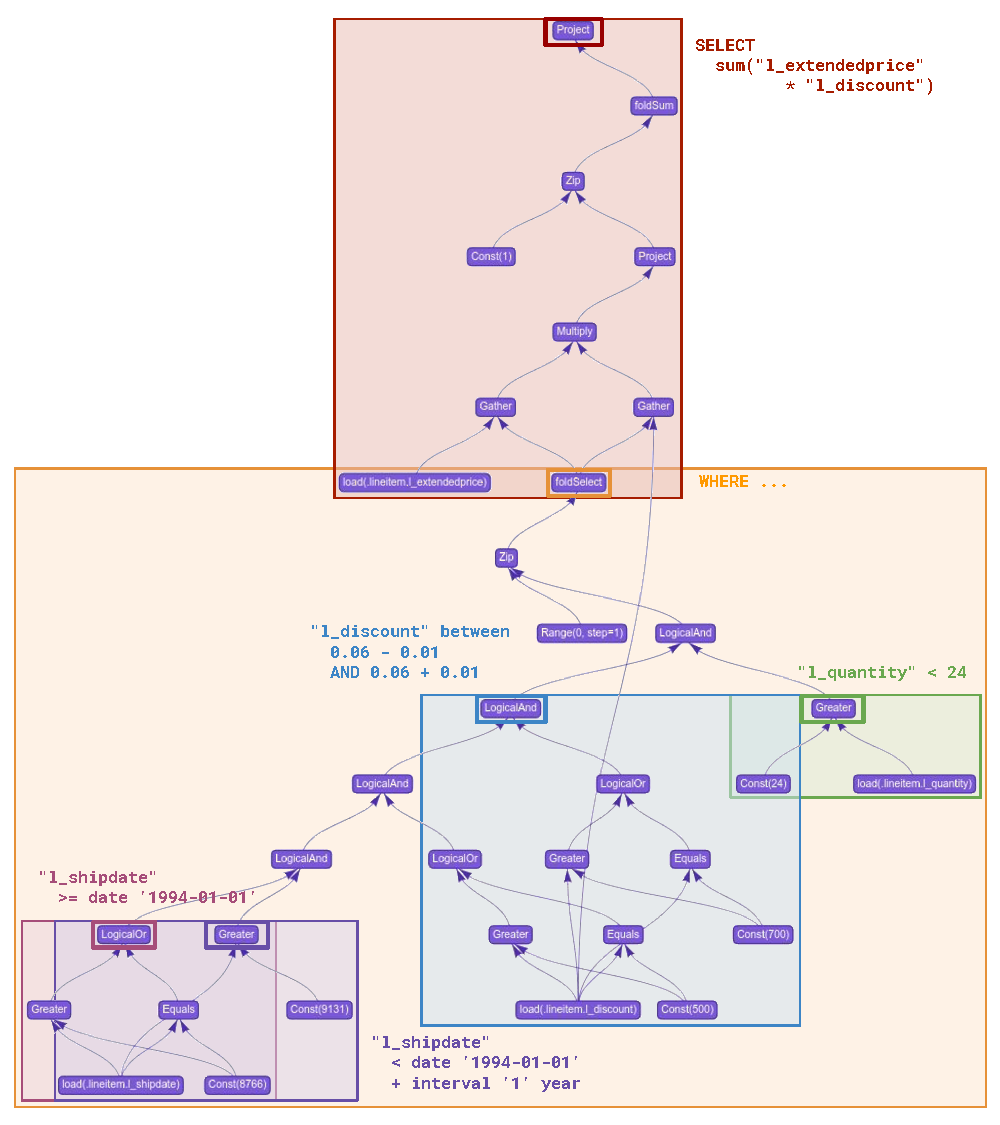
\includegraphics[width=0.95\linewidth]{appendix/q6-voodoo.pdf}
    \caption{Voodoo vector expressions generated for TPC-H query 6}
    \label{fig:q6-voodoo}
\end{figure}

\chapter{The Apache Calcite Framework}
\label{appendix:calcite}

\subsubsection{Architecture of Apache Calcite}

\begin{figure}[H]
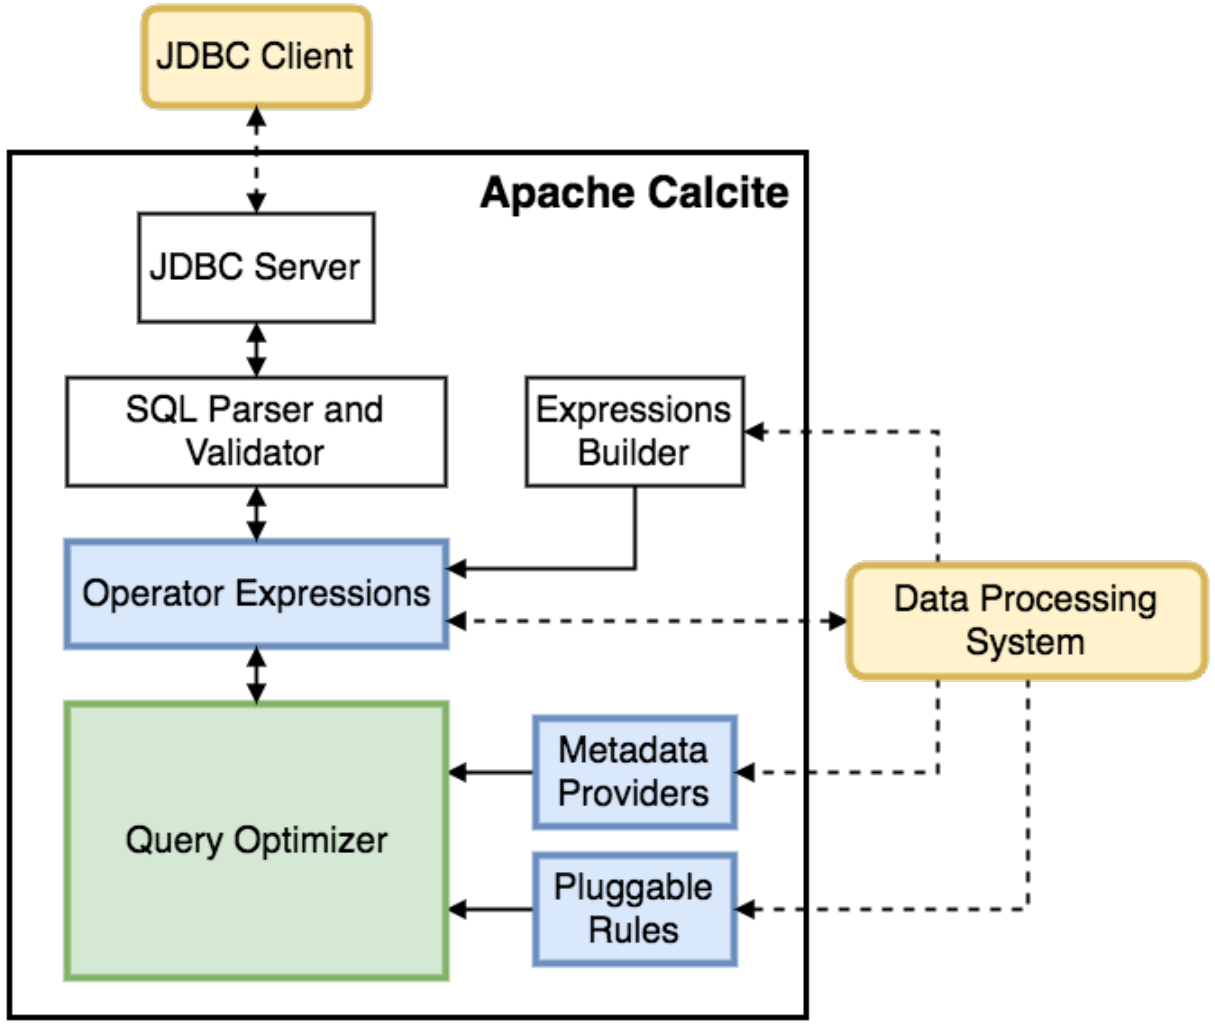
\includegraphics[width=0.4\textwidth]{appendix/calcite-architecture.png}
\centering
\caption{Architecture of Apache Calcite \cite{Begoli:2018:ACF:3183713.3190662}}
\label{fig:calcite-architecture}
\end{figure}

Calcite consists of most of the components needed to make a DBMS, with three significant omissions: algorithms to process data, storage of data, and a catalog for metadata. Figure \ref{fig:calcite-architecture} shows an overview of its architecture and interactions.

Firstly, Calcite provides a JDBC server (\emph{Avatica}), as well as a default implementation of its SPI. Alternatively, an application can use Avatica's JDBC driver directly (which is the approach we take with our web-interface).

Calcite then supports query evaluation in each of the following stages:
\begin{enumerate}
    \item \textbf{Parsing} the SQL query. Calcite provides an LL($k$) parser generated by JavaCC, and developers usually need not consider this step beyond setting some basic configuration options.
    \item \textbf{Validating} the SQL query. Calcite validates queries against any known metadata. Developers need to provide an interface that allows Calcite to get this metadata for a table (an \emph{adapter}).
    \item \textbf{Optimising} the logical plan, and converting it to physical expressions. Calcite can do this with some help. It provides two algorithms for rule-based logical query optimisation, as well as around one-hundred rules. However, developers will likely need to add further rules, including rules to rewrite a logical plan into physical expressions for their application.
    \item \textbf{Executing} the physical plan, by converting it into application-specific executions. Calcite can handle this in simple cases, say where the application actually supports SQL input (i.e. Calcite is just being used as an optimiser). In other cases, such as ours, this step requires a lot of application-specific code to be written.
\end{enumerate}

\subsubsection{Relational algebra}
\label{rel}

Calcite uses relational algebra \cite{Codd:1970:RMD:362384.362685} to express queries. Specifically, it builds a tree of \texttt{RelNode}s, each of which represent a relational operator. Each \texttt{RelNode} could represent, for example, a \texttt{TableScan}, \texttt{Project}, \texttt{Filter}, \texttt{Aggregate}, \texttt{Join}, \texttt{Union}, \texttt{Intersect} or \texttt{Sort}.

Projection and sort fields, as well as filter and join conditions, are expressed by trees of \texttt{RexNode}s. A \texttt{RexNode} represents a row-level expression, and its implementations include \texttt{RexCall} (an operation such as "add" or "is equal to"), \texttt{RexInputRef} (a reference to an input column) and \texttt{RexLiteral} (a literal value), as well as many others (which we do not consider).

Relational expressions are associated with \emph{traits} (\texttt{RelTrait}s), which describe their physical properties, such as ordering, grouping, or partitioning. The most important trait, however, is the \emph{calling convention} (\texttt{Convention}), which specifies the data processing system where the expression will be executed. The \texttt{Logical} calling convention is used when no implementation has been selected.

\subsubsection{Query processing and optimisation}

Calcite includes \emph{planner rules} (\texttt{RelOptRule}s) to transform expression trees. Each rule defines a condition on the original tree, and a conversion, that rewrites part of the tree. Calcite provides common rules, such as the \texttt{FilterIntoJoinRule}, which pushes a filter into a join where possible, to reduce the work in the join. Developers also must provide their own rules to transform the tree from a logical to an optimised physical plan.

Calcite also provides two planner engines (\texttt{RelOptPlanner}s) to apply these rules: one requires a cost-model and uses a dynamic programming algorithm, similar to Volcano's \cite{Graefe:1994:VEP:627290.627558} (\texttt{VolcanoPlanner}), whilst the other exhaustively applies rules until it reaches a fixpoint (\texttt{HepPlanner}).

\subsubsection{Adapters}

\begin{figure}[H]
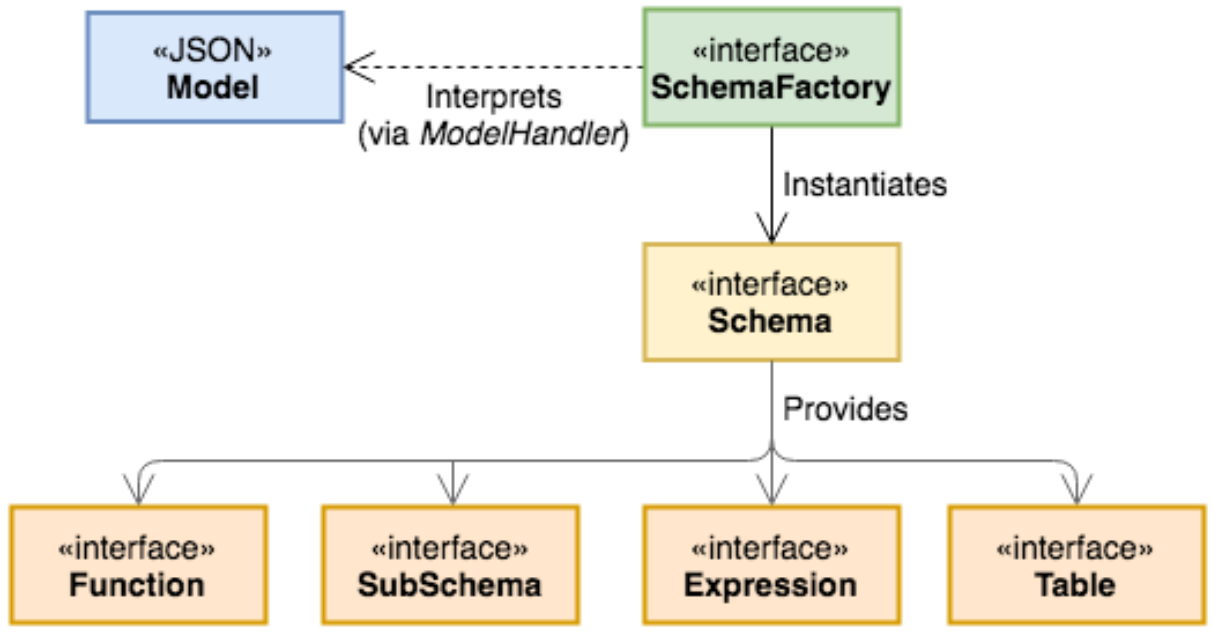
\includegraphics[width=0.42\textwidth]{appendix/calcite-adapter.png}
\centering
\caption{A minimal adapter for Apache Calcite \cite{Begoli:2018:ACF:3183713.3190662}}
\label{fig:calcite-adapter}
\end{figure}

As Calcite does not include a storage layer, it requires developers to build an \emph{adapter}. Figure \ref{fig:calcite-adapter} shows the design of a minimal adapter:
\begin{itemize}
    \item The \texttt{Model} is a JSON-formatted description of the physical properties of the data source being accessed.
    \item The \texttt{Schema} is a definition of the data found in the model, and is generated by a \texttt{SchemaFactory} for the adapter. Usually this will use a \texttt{TableFactory}, which generates a \texttt{Table} defining the names and types of the columns in each table, as well as any statistics available, such as cardinalities, distributions, and which columns are keys.
\end{itemize}

An adapter also usually provides a set of rules to be added to the planner. Specifically, rules to rewrite logical operators to physical operators of the adapter's convention.

The minimal rule set includes a translation for table-scans, which implement the access paths for tables in the adapter. Once Calcite can read the data, it can implement all other operators using the \texttt{Enumerable} calling convention, which uses a conventional iterator implementation written in Java.

Rules are also used to convert all other operators, to avoid plans relying too heavily on costly \texttt{Enumerable} operators. Each of these rules, in our case, defines an implementation instead using the \texttt{Voodoo} convention.

\chapter{Relational Operator Implementations}
\label{appendix:rel}

\begin{enumerate}
    \item \textbf{Table scans}
    
    \texttt{TableScan} is a relatively simple operator that can access a \texttt{VoodooTable}, and \texttt{Import}, \texttt{Persist} and \texttt{Load} its column vectors into the back-end's memory.
    
    \item \textbf{Projections}
    
    \texttt{Project} is a similarly simple operator. Each projected field is defined as a row expression and is implemented as described in subsection \ref{sub:rex}. The final result is then made available for the parent node to access.
    
    \item \textbf{Filters}
    
    \begin{figure}
        \centering
        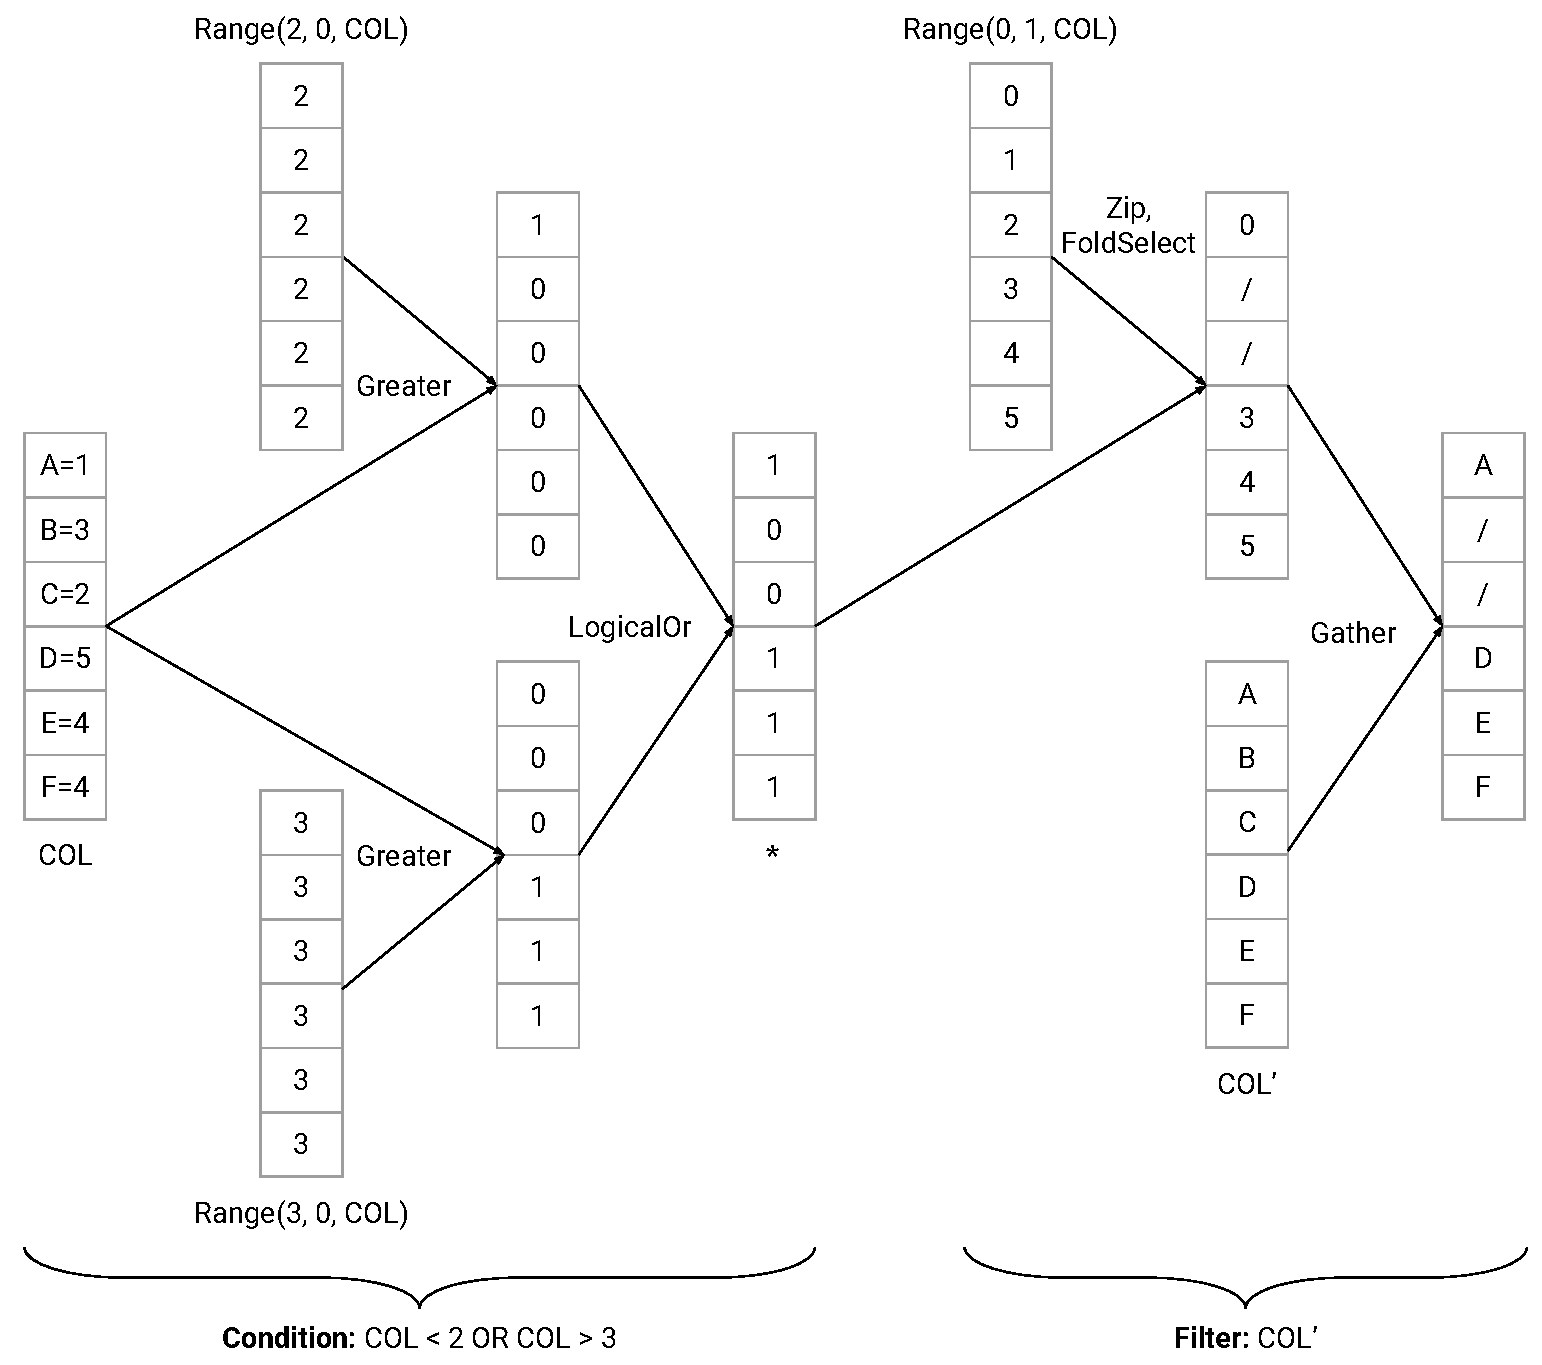
\includegraphics[width=0.75\linewidth]{appendix/filter.pdf}
        \caption{Implementing $\sigma_{\text{COL} < 2 \lor \text{COL} > 3}$ in Voodoo vector algebra}
        \label{fig:filter}
    \end{figure}
    
    \texttt{Filter} represents a selection in relational algebra. To implement a filter, we first implement its condition, which is a row expression. This should return a vector of zeroes and ones, where the ones correspond to rows which should be selected. Figure \ref{fig:filter} shows an example of this, where we have reached the vector labelled "$*$". We \texttt{Zip} this condition vector with the row indices of the table. We then use a \texttt{FoldSelect}, which selects the indices corresponding to non-zero values in the condition vector. These indices are then used to \texttt{Gather} the selected rows from each column of the table.
    
    \item \textbf{Aggregates}
    
    
    
    \item \textbf{Joins}
    
    
\end{enumerate}

\chapter{Voodoo API Implementation}
\label{appendix:api}

\begin{enumerate}

\item \texttt{Import(vector v1)}

This loads a vector holding input data (in the form of a pointer to a buffer) into the VectorProcessor. This vector is now referred to as a persistent or input vector.

\item \texttt{Load(vector v1)}

This loads a previously created persistent vector and allows other calls to access the data held within it. It registers the persistent vector as being present in the parameters to the final fragment. 

This generates a Clang::ParmVarDecl declaring the name and type of the vector in the fragments function parameters.

\item \texttt{Project(vector v1, KeyPath k1)}

This projects a loaded vector and allows other calls to access the data held within it. It leads to the generation of the dominating iterator for loop that is used to cycle through the values of the projected vector. If the vector v1 contains multiple members, then KeyPath k1 is used to access the specific member, otherwise it is ignored.

This generates a Clang::DeclStmt declaring and initialising the vector e.g. "tmp1 = v1[dominatingIterator].k1"

\item \texttt{Gather(vector v1, positions)}

Gather is a more complicated version of project. Instead of cycling through all the values of a vector it takes in another vector (positions) which it uses as the indices of the vector to access. 

This generates a Clang::DeclStmt declaring and initialising the vector e.g. "tmp1 = v1[positions[dominatingIterator]]"

\item \texttt{LogicalAnd(vector v1, v2)}, \texttt{LogicalOr(vector v1, v2)}, \texttt{BitwiseAnd(vector v1, v2)}, \texttt{BitiwseOr(vector v1, v2)}, \texttt{Equals(vector v1, v2)}, \texttt{Add(vector v1, v2)}, \texttt{Subtract(vector v1, v2)}, \texttt{Greater(vector v1, v2)}, \texttt{Modulo(vector v1, v2)}, \texttt{Divide(vector v1, v2)} 
All of these Voodoo API calls take two vectors of identical size and perform a single operation on them, outputing a single vector of the same size. 

This generates a Clang::DeclStmt declaring and initialising the vector e.g. "tmp1 = v1 (+ / - / * / == / ...) v2"

\item \texttt{BitShift(vector v1, v2)}

This take two vectors of identical size and shifts the first by the second amount. If the amount is positive it is a right shift otherwise it is a left shift. This outputs a single vector of the same size.

\item \texttt{Range(int/long/float min, count, step)}

Range generates a vector of size count, representing a range of numbers, starting at min and increasing by count between each number. Count can also be input as a vector, and range will generate a vector of identical size to count. 

This generates a Clang::DeclStmt declaring and initialising the vector e.g. "tmp1 = min + step * dominatingIterator"

\item \texttt{Zip(vector v1, v2, KeyPath k1, k2)}

Zip takes two vectors of identical size and zips them together into one vector. The output vector will contain vector v1 in KeyPath k1 and vector v2 in KeyPath k2. This is necessary for the fold operations, which require a zipped vector, and utilise KeyPath to access them.

This generates a Clang::DeclStmt declaring and initialising the vector e.g. "tmp1 = \{{k1: v1, k2: v2\}}"

\item \texttt{FoldSelect(vector v1, KeyPath fold, val)}

foldSelect takes a vector and branches via an if statement based on the val of the vector. Returning v1.fold if v1.val is non-zero, otherwise returning -1. Any further statements using the output of the foldSelect will be placed inside the if statement.

This generates multiple Clang::Stmts, generating the output of the foldSelect and the branch "tmp4 = tmp3.value ? tmp3.fold : -1;
if (tmp3.value) \{{ ... \}}"

\item \texttt{FoldSum(vector v1, KeyPath fold, val)}, \texttt{FoldMax(vector v1, KeyPath fold, val)}, \texttt{FoldMin(vector v1, KeyPath fold, val)}

foldSum/Max/Min takes a vector and computes the sum / max / min of the val based on the fold attribute. This generates a Clang::Stmt assigning 
"tmp7 = tmpAggregate6[tmp5.fold] = tmpAggregate6[tmp5.fold] + tmp5.value;"

This will "reduce" a vector to a single value. 

\item \texttt{Cross(vector v1, v2)}

Cross generates a nested for loop, looping through the values of v2. This allows data from one table to be crossed with another table. During the fragment generation process this manifests as a fragment contained within another fragment.

This generates a Clang::Stmt declaring the for loop "for(int dominatingIteratorOffset2 = 0; i < v2.size; i++) \{{...\}}" and allows future calls to access the new iterator to loop through the values of v2.

\item \texttt{ReturnVector(vector v1)}

\texttt{ReturnVector} projects a vector into a new output vector with a buffer to hold the final output values. This adds the output vector to the parameter list so the buffer location can specified at runtime by the \texttt{VectorProcessor}. This invokes the fragment generation code and generates the final code to be run in addition to the output size and type, storing it in the vector. This generates a \texttt{Clang::Stmt} assigning the vector e.g. "persistent1[0] = v1" or "persistent1[dominatingIterator] = v1" and a \texttt{Clang::ParmVarDecl} declaring the name and type of the vector in the fragments function parameters. This returns the vector, ready to be resolved (ran) and for the values to be read.

\item \texttt{ReturnMultiVector(list of vectors vs)}

This generates multiple return statements, adding each return statement to the fragment as well as each output buffer and then generating the code for this fragment. The final code is stored in the first vector. When the list of vectors is resolved, only the first vector is run, but all output buffers from the list are registered to OpenCL and so all output vectors are populated. 

This returns a list of vectors, ready to be resolved and for the values of each vector to be read.

\item \texttt{Resolve(vector or list of vectors)}

This runs the given vectors, passing input and output buffers to the \texttt{VectorProcessor} and then returning the vectors containing the results back to the user.\\
 This call will only work on vectors produced from previous calls to \texttt{ReturnVector} or \texttt{ReturnMultiVector}.\\
Once the relevant Clang statements have been created, they are added to the \texttt{AstVector}. The \texttt{AstVector} also stores the \texttt{AstVectors} that this function requires.

\end{enumerate}

\chapter{Usage}

Combine \url{https://gitlab.doc.ic.ac.uk/voodoo-project/Voodoo/blob/master/README.md} and \url{https://gitlab.doc.ic.ac.uk/voodoo-project/calcite/blob/voodoo/voodoo/README.md} with screenshots to demonstrate usage...

\chapter{Metrics}
\label{appendix:metrics}

\section{Test Coverage}

\begin{figure}[H]
    \centering
    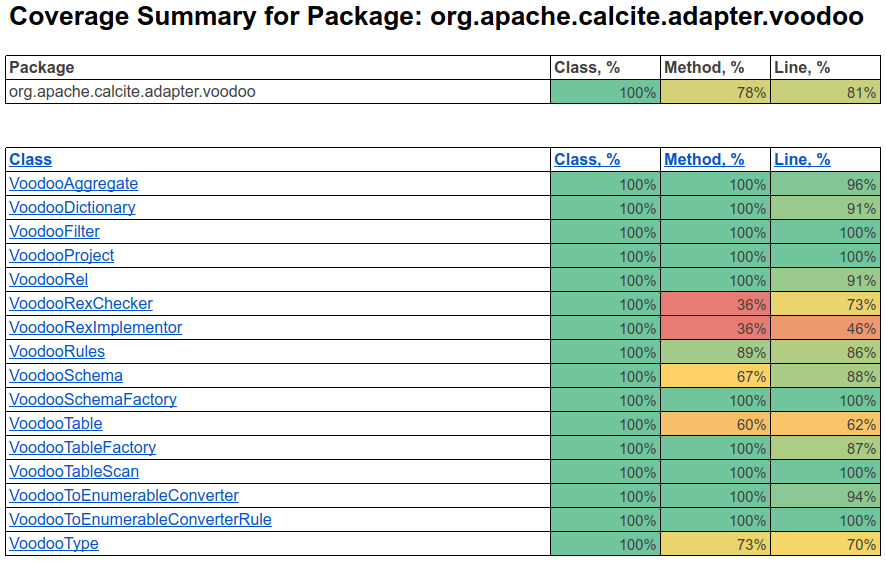
\includegraphics[width=0.7\linewidth]{evaluation/frontend-coverage.png}
    \caption{Font-end test coverage}
    \label{fig:fontend-cov}
\end{figure}

\begin{figure}[H]
    \centering
    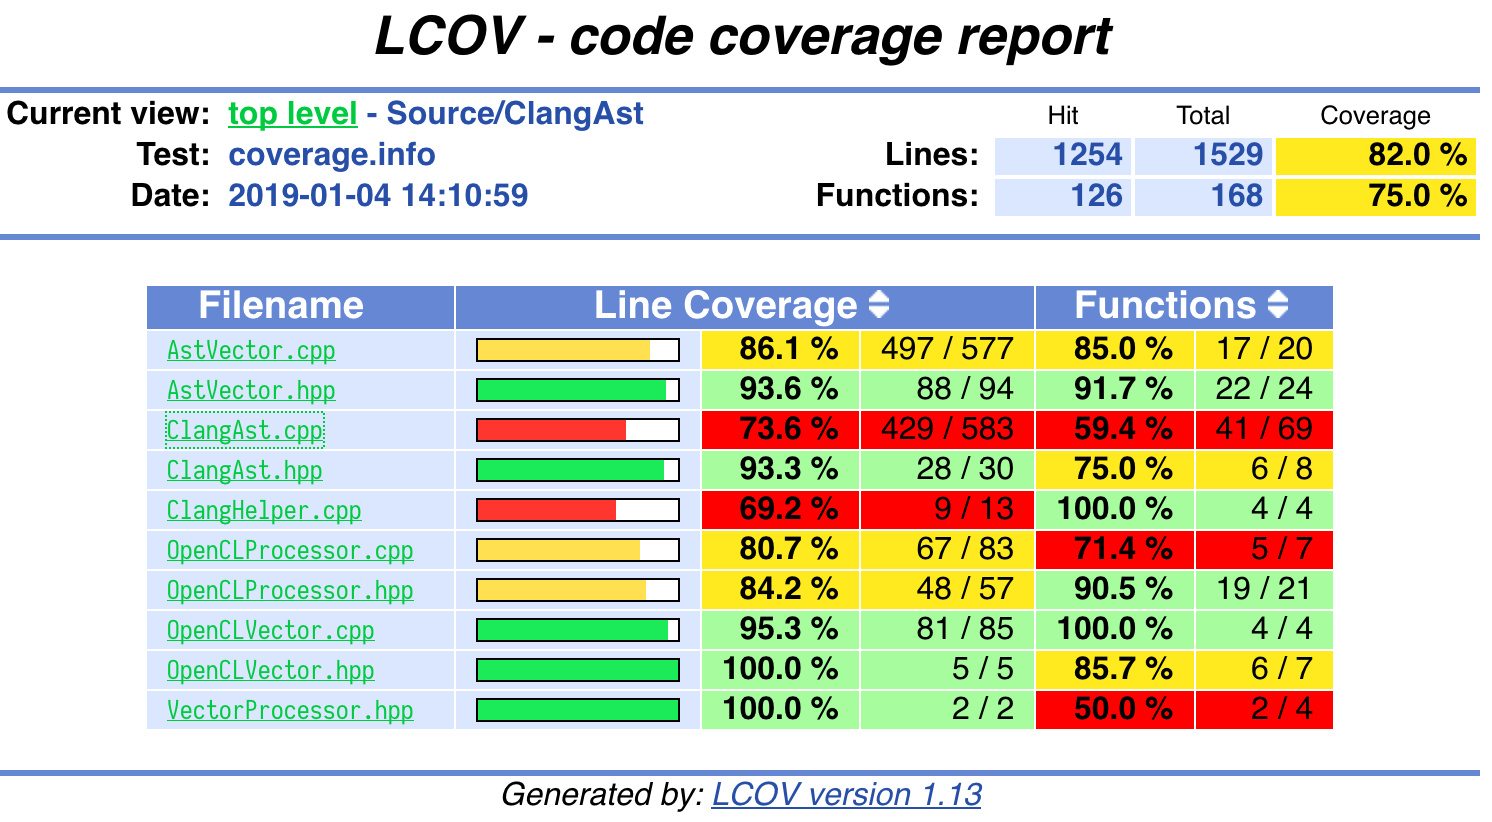
\includegraphics[width=0.75\linewidth]{evaluation/backend-coverage.png}
    \caption{Back-end test coverage.}
    \label{fig:backend-cov}
\end{figure}

\section{\texttt{Metrix++} results}

\begin{table}[H]
    \centering
    \begin{tabular}{@{}lllll@{}}
        \toprule
        \textbf{Metric}       & \textbf{Max} & \textbf{Avg} & \textbf{Total} \\ \midrule
        Cyclomatic Complexity & 71           & 1.29         & 1760           \\
        Maximum Indentation   & 11           & 1.41         & 1925           \\
        Magic Numbers         & 179          & 4.28         & 1341           \\ \bottomrule
    \end{tabular}
    \caption{\label{table:original-metrics}Original code results}
\end{table}

\begin{table}[H]
    \centering
    \begin{tabular}{@{}lllll@{}}
        \toprule
        \textbf{Metric}       & \textbf{Max} & \textbf{Avg} & \textbf{Total} \\ \midrule
        Cyclomatic Complexity & 71           & 1.86         & 820           \\
        Maximum Indentation   & 5            & 1.42         & 624            \\
        Magic Numbers         & 15           & 3.02         & 348           \\ \bottomrule
    \end{tabular}
    \caption{\label{table:opencl-metrics}\texttt{OpenCL} implementation results}
\end{table}

\begin{table}[H]
    \centering
    \begin{tabular}{@{}lllll@{}}
        \toprule
        \textbf{Metric}       & \textbf{Max} & \textbf{Avg} & \textbf{Total} \\ \midrule
        Cyclomatic Complexity & 24           & 1.05         & 128            \\
        Maximum Indentation   & 6            & 1.66         & 202           \\
        Magic Numbers         & 25           & 3.03         & 100           \\ \bottomrule
    \end{tabular}
    \caption{\label{table:clangast-metrics}\texttt{ClangAst} implementation results}
\end{table}

\paragraph{Disclaimer} These values should be taken with a pinch of salt. There are significant differences between the implemented algorithms, and different style choices were made.

Furthermore, the metric \emph{Magic Numbers} includes \textbf{0}s and \textbf{1}s and we do not know how \texttt{Metrix++} implements cyclomatic complexity.

\chapter{Dependencies}

\begin{table}[h]
    \centering
    \begin{tabular}{l l l}
        \hline
        \textbf{Repository} & \textbf{Dependency} & \textbf{License} \\
        \hline
        \texttt{calcite}    & Apache Calcite & Apache License 2.0 \\
        \texttt{calcite}    & Guava          & Apache License 2.0 \\
        \texttt{calcite}    & JUnit          & Eclipse Public License 1.0 \\
        \texttt{calcite}    & sqlline        & 3-Clause BSD License \\ 
        \hline
        \texttt{voodoo}     & Clang          & University of Illinois/NCSAOpen Source License \\
        \texttt{voodoo}     & OpenCL         & Khronos Specific License \\
        \texttt{voodoo}     & Boost          & Boost Software License \\
        \texttt{voodoo}     & Googletest          & 3-Clause BSD License \\
        \hline
        \texttt{voodoo-vis} & Axios          & MIT License \\
        \texttt{voodoo-vis} & Buefy          & MIT License \\
        \texttt{voodoo-vis} & Codemirror     & MIT License \\
        \texttt{voodoo-vis} & VisJS          & May be distributed under MIT or Apache 2.0 \\
        \texttt{voodoo-vis} & VueJS          & MIT License \\
        \hline
    \end{tabular}
    \caption{\label{table:dependencies}Licenses for each library used}
\end{table}


All software and packages detailed above are under licenses which would allow commercial use.

If this project was to be open-sourced, any copies of packages must include the original copyright texts and licenses (should we choose to distribute them along with our own source).

\chapter{Clang AST for the Simple Query}

\begin{figure}[p]
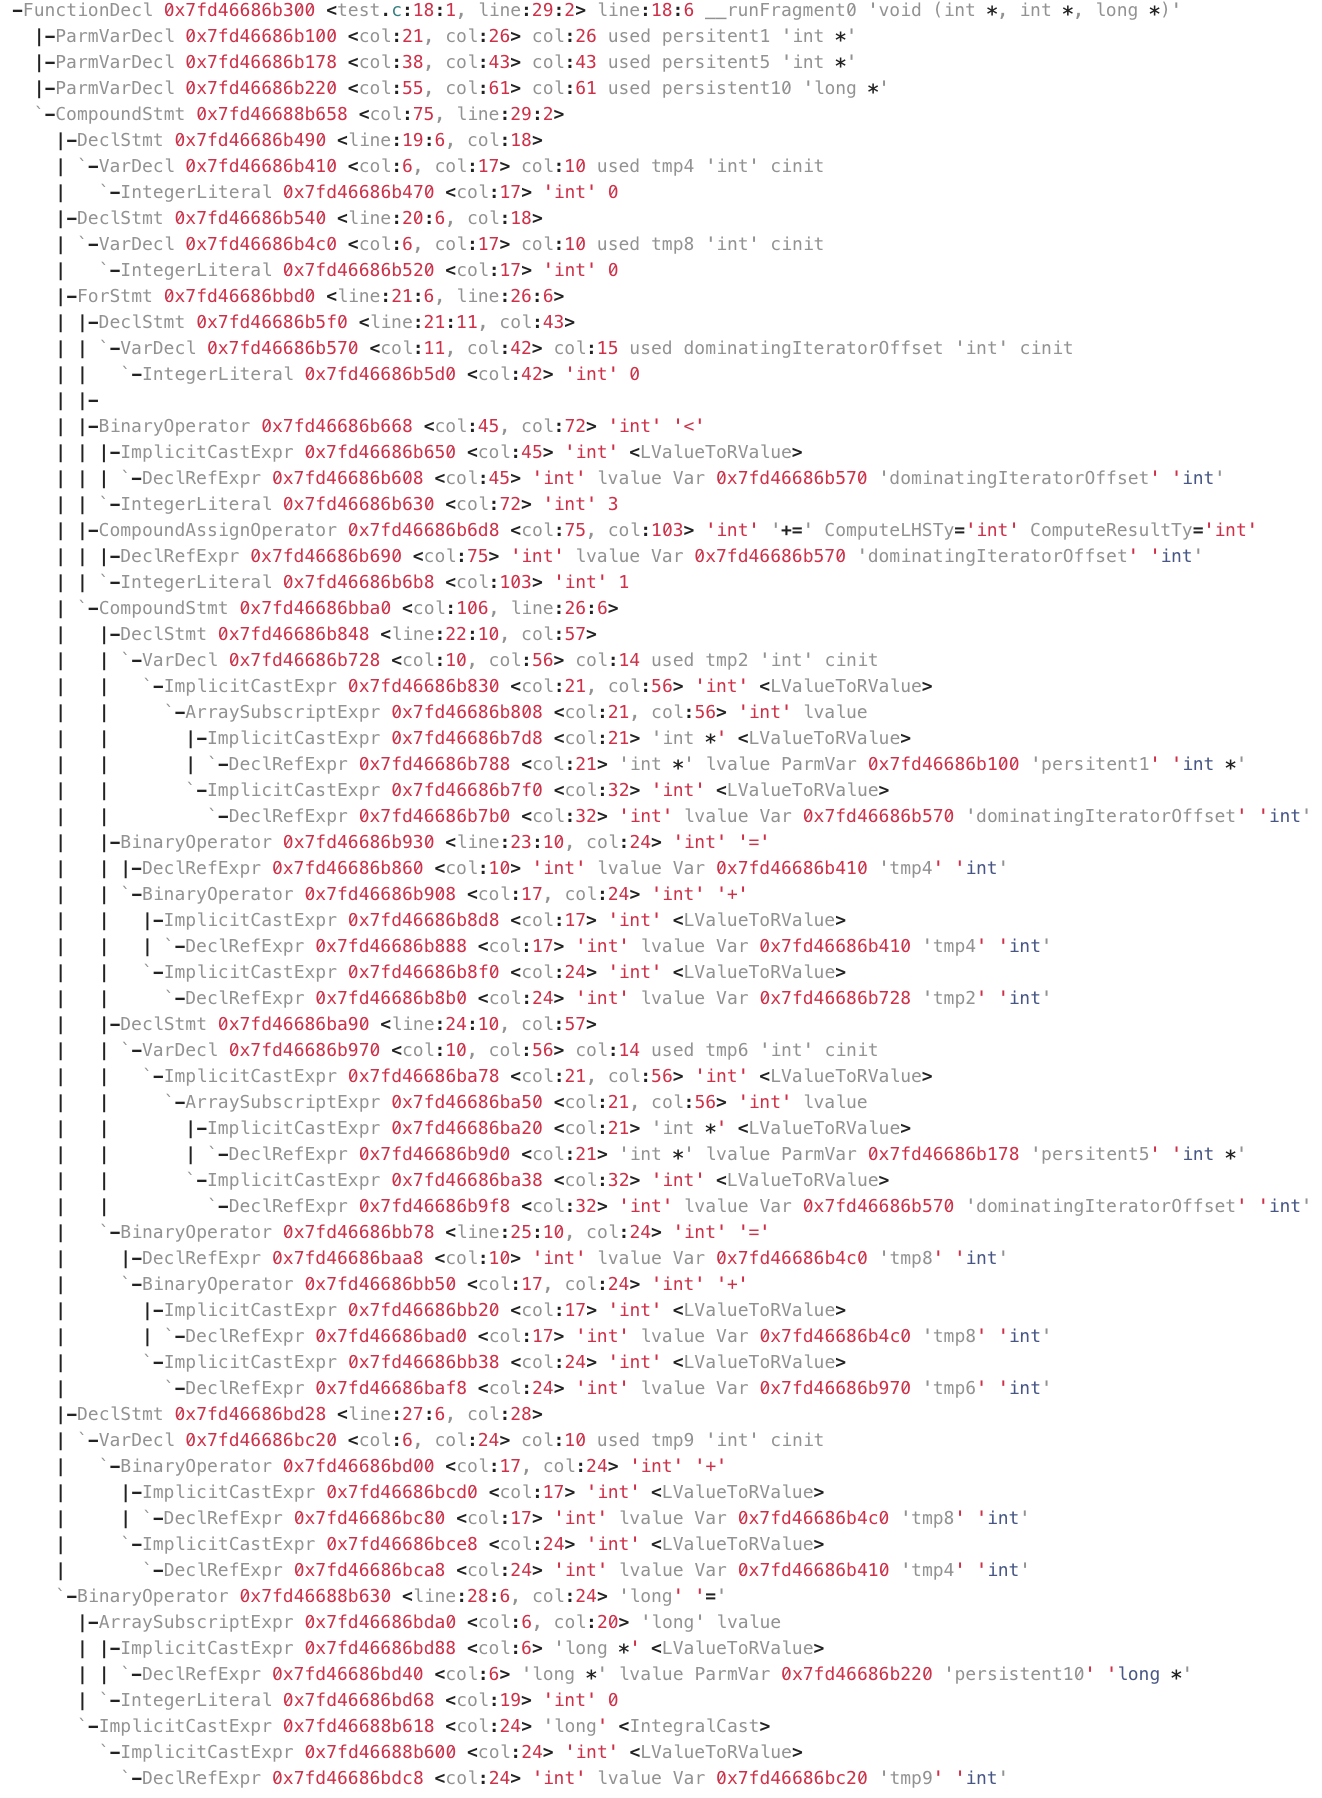
\includegraphics[width=0.99\textwidth]{appendix/ClangAstSimpleQuery.png}
\centering
\caption{Clang AST for Simple Query}
\label{fig:clangast}
\end{figure}

\chapter{Generating Fragments for FoldSelect}

Dealing with the foldSelect fragment is slightly different as it creates an if statement instead of a typical for loop statement. Any calls following the foldSelect will be inserted inside the if statement. 

If a reducer is called in the foldSelect scope, this needs to close the if statement (if it is a nested foldSelect, then close all the if statements) and then close the for loop the statement belongs in. Figure \ref{fig:fragmentConstructionfoldSelect} shows a step by step process of how the fragments are created for the query in figure \ref{fig:ASTfoldSelect}. All folds require a zip and a range call before they can be used. These calls have been omitted for brevity.

\begin{figure}
\centering
\begin{subfigure}{0.9\textwidth}
  \centering
  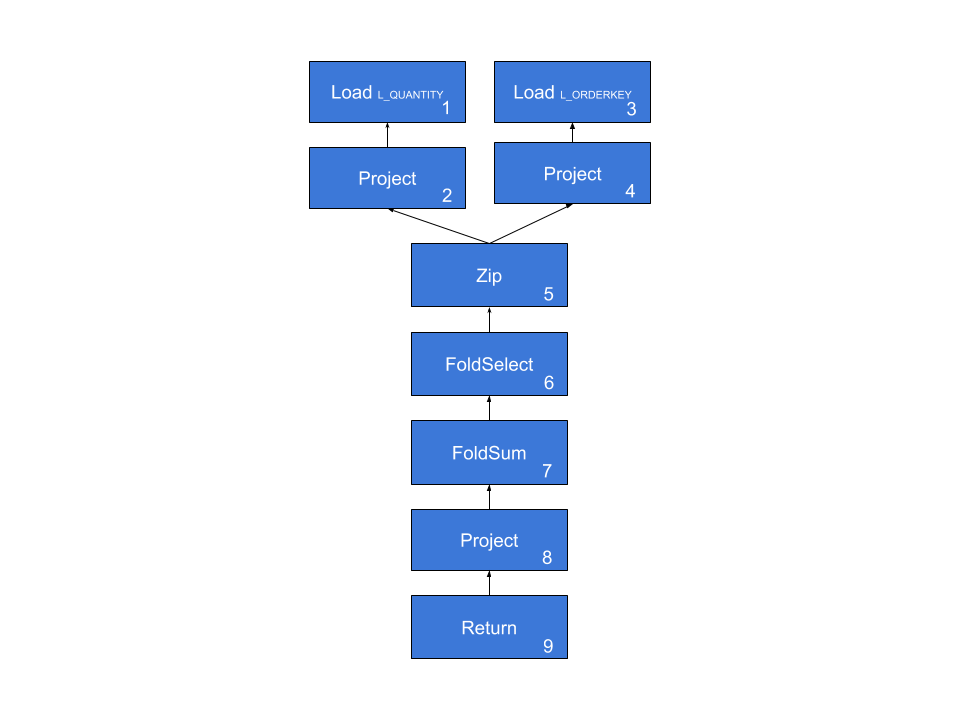
\includegraphics[width=1\linewidth]{appendix/foldSelectQuery.png}
  \caption{AST of a foldSelect Query}
  \label{fig:ASTfoldSelect}
\end{subfigure}%

\begin{subfigure}{0.95\textwidth}
  \centering
  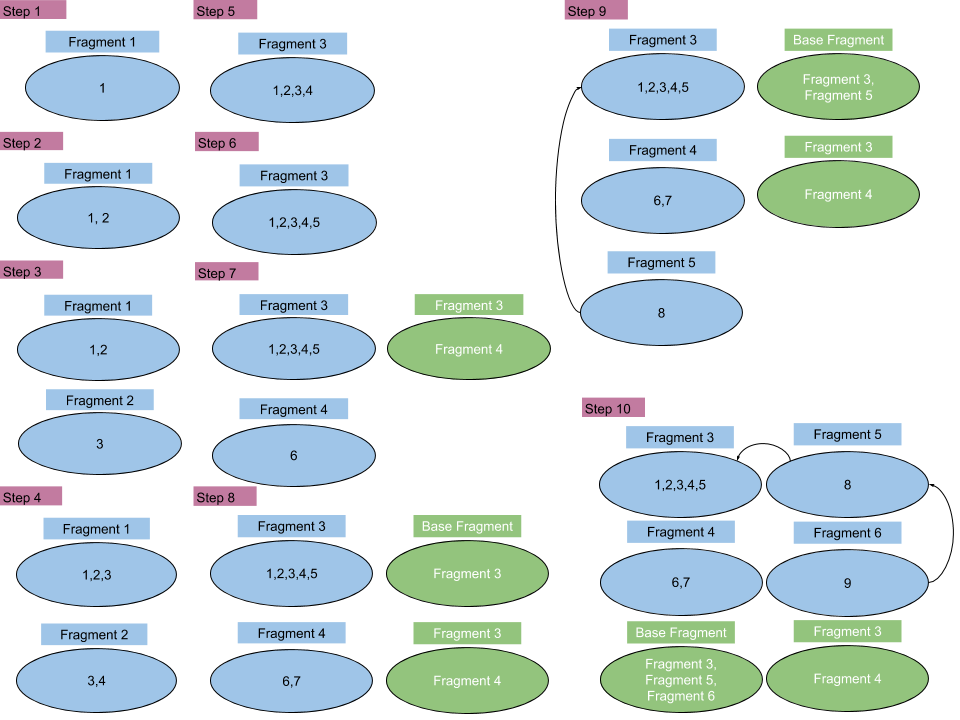
\includegraphics[width=1\linewidth]{appendix/FragmentConstructionFoldSelect.png}
  \caption{Fragment Construction for \ref{fig:ASTfoldSelect}}
  \label{fig:fragmentConstructionfoldSelect}
\end{subfigure}
\caption{Fragment Construction for a foldSelect Query}
\label{fig:foldSelectQuery}
\end{figure}

\begin{figure}
\begin{lstlisting}[frame=single, language=C]
__kernel void __runFragment0(
    __global int *persitent1, // L_QUANTITY column vector
    __global int *persitent3, // L_ORDERKEY column vector
    __global long *persistent10 // Result vector
) {
    struct {
        int fold;
        int value;
    } tmp5;
    int tmp6;
    int tmpAggregate7[32767] = {};
    int tmp8 = 0;
    for (int dominatingIteratorOffset = 0; 
         dominatingIteratorOffset < 3; 
         dominatingIteratorOffset += 1) {
        int tmp2 = persitent1[dominatingIteratorOffset];
        int tmp4 = persitent3[dominatingIteratorOffset];
        {
            tmp5.fold = tmp2;
            tmp5.value = tmp4;
        }
        {
            tmp6 = tmp5.value ? tmp5.fold : -1;
            if (tmp5.value) {
                tmp8 = tmpAggregate7[tmp6] = tmpAggregate7[tmp6] + tmp6;
            }
        }
    }
    int tmp9 = tmp8;
    persistent10[0] = tmp9;
}
\end{lstlisting}
    \caption{OpenCL code for \ref{fig:foldSelectQuery}}
    \label{fig:opencl-code}
\end{figure}

\chapter{A Dynamic Programming Algorithm for Generating Fragments}
\label{appendix:dpalgo}

The current implementation assumes that at each stage


\begin{figure}
    \centering
    \begin{subfigure}{0.5\linewidth}
        \centering
        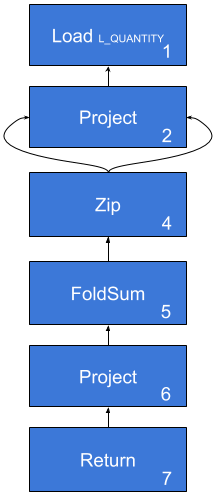
\includegraphics[width=0.5\linewidth]{appendix/DPExplain.png}
        \caption{}
        \label{fig:DPSimpleQuery}
    \end{subfigure}
    \begin{subfigure}{\linewidth}
        \centering
        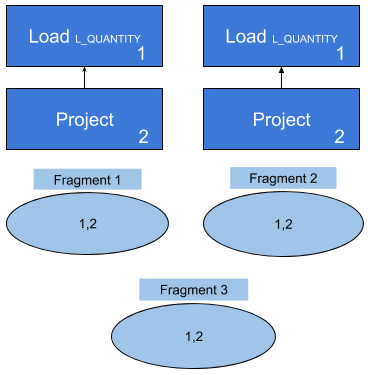
\includegraphics[width=0.5\linewidth]{appendix/DPExplainFrag.png}
        \caption{The process of creating fragments and merging fragments using the recursive solution before the zip statement can be added}
        \label{fig:DPSimpleQueryFrag}
    \end{subfigure}
    \caption{Caption}
    \label{fig:my_label}
\end{figure}